\documentclass[12pt]{article}
\usepackage{setspace}
\usepackage{extsizes}
\usepackage{float}
\usepackage{amsmath, amsthm, amssymb}    
\usepackage[margin=.5in]{geometry}
\usepackage{tikz}
\usepackage{pgfplots}
\pgfplotsset{compat=1.13}
\usepackage{tkz-euclide}
\usepackage{bclogo}
\usepackage{graphicx}


\title{\vspace{-2.0cm}Homework 9}
\author{Joanne Wardell}
\date{Tuesday, October 2, 2018}
\begin{document}
\maketitle

\subsection*{Section 14.7}
\noindent 2.) $f(x,y) = 2xy-5x^{2}-2y^{2}+4x + 4y -4$\\\\
\noindent $\frac{\partial f}{\partial x} = -8x + 4$, \hspace{10pt} $\frac{\partial ^{2} f}{\partial x^{2}} = -8$\\\\
\noindent $\frac{\partial f}{\partial y} = -2y + 4$, \hspace{10pt} $\frac{\partial ^{2} f}{\partial y^{2}} = -2$\\\\
\noindent $\frac{\partial^{2} f}{\partial x \partial y } = \frac{\partial }{\partial x}[-2y + 4] = 0$\\\\
\noindent $\mathbf{H} = f_{xx}f_{yy} - f_{yx}^{2} = 16 > 0$\\\\
\noindent $-8x + 4 = 0 \rightarrow x = 2$\\\\
\noindent $-2y + 4 = 0 \rightarrow y = 2$\\\\
\noindent $f(2, 2) = -8$ is a \textbf{local maximum} since $f_{x}(2, 2) > 0$, $f_{y}(2, 2) > 0$, and $\mathbf{H}\Big|_{(2,2)} > 0$.\\\\
\noindent 10.) $f(x, y) = x^{2} + 2xy$\\\\
\noindent $\frac{\partial f}{\partial x} = 2x + 2y$, \hspace{10pt} $\frac{\partial ^{2} f}{\partial x^{2}} = 2$\\\\
\noindent $\frac{\partial f}{\partial y} = 2x$, \hspace{10pt} $\frac{\partial ^{2} f}{\partial y^{2}} = 0$\\\\
\noindent $\frac{\partial^{2} f}{\partial x \partial y } = \frac{\partial }{\partial x}[2x] = 2$\\\\
\noindent $\mathbf{H} = f_{xx}f_{yy} - f_{yx}^{2} = -4 < 0$\\\\
\noindent $2x+2y = 0$\\\\
\noindent $2x=0= 0 \rightarrow x = 0 \rightarrow y = 0$\\\\
\noindent $f(0, 0) = 0$ is a \textbf{saddle point} since $\mathbf{H}\Big|_{(0,0)} < 0$.\\\\
\noindent 14.) $f(x,y) = x^{3}+3xy + y^{3}$\\\\
\noindent $\frac{\partial f}{\partial x} = 3x^{2} + 3y$, \hspace{10pt} $\frac{\partial ^{2} f}{\partial x^{2}} = 6x$\\\\
\noindent $\frac{\partial f}{\partial y} = 3x + 3y^{2}$, \hspace{10pt} $\frac{\partial ^{2} f}{\partial y^{2}} = 6y$\\\\
\noindent $\frac{\partial^{2} f}{\partial x \partial y } = \frac{\partial }{\partial x}[3x + 3y^{2}] = 3$\\\\
\noindent $3x^{2} + 3y = 0 $\\
\noindent $3x^{2} = -3y \rightarrow y = -x^{2}$\\\\
\noindent $3x + 3y^{2} = 0$\\
\noindent $3x + 3(-x^{2})^{2} = 0$\\
\noindent $3x = -3x^{4}$\\
\noindent $x^{-4}[x = -x^{4}]$\\
\noindent $x^{3}[x^{-3} = -1]$\\
\noindent $-1 = x^{3} \rightarrow x = -1$\\\\
\noindent $y = -((-1)^{2}) = -1$\\\\
\noindent $\mathbf{H} = f_{xx}f_{yy} - f_{yx}^{2} = 36 - 9 > 0$\\\\
\noindent $f(-1, -1) = 1$ is a \textbf{local maximum} since $f_{x}(-1, -1) < 0$, $f_{y}(-1, -1) < 0$, and $\mathbf{H}\Big|_{(2,2)} > 0$.\\\\
\noindent 30.) $f(x, y) = \ln(x + y) + x^{2}-y$\\\\
\noindent $\frac{\partial f}{\partial x} = \frac{1}{x+y} + 2x$, \hspace{10pt} $\frac{\partial ^{2} f}{\partial x^{2}} = -\frac{1}{(x + y)^{2}} + 2$\\\\
\noindent $\frac{\partial f}{\partial y} = \frac{1}{x + y} -1 $, \hspace{10pt} $\frac{\partial ^{2} f}{\partial y^{2}} = -\frac{1}{(x + y)^{2}}$\\\\
\noindent $\frac{\partial^{2} f}{\partial x \partial y } = \frac{\partial }{\partial x}[\frac{1}{x+y} -1 ] = -\frac{1}{(x + y)^{2}}$\\\\
\noindent $\frac{1}{x + y} + 2x= 0 $\\
\noindent $\frac{(x + y)}{-2x}[\frac{1}{x + y} = -2x]$\\
\noindent $y = -2x^{-1} - x$\\\\
\noindent $\frac{1}{x + y} = 0$\\
\noindent $\frac{1}{x  -2x^{-1} -x} = 0 \rightarrow x = 0$\\\\
\noindent $y = 0$\\\\
\noindent $\mathbf{H} = f_{xx}f_{yy} - f_{yx}^{2} = 0$\\\\
\noindent Since $\mathbf{H} = 0$, nothing can be concluded about $f(0, 0)$.\\\\
\noindent 32.) $D(x, y) = x^{2} - xy +y^{2} + 1$, \hspace{10pt} $x = 0$, \hspace{10pt} $y = 4$, \hspace{10pt} $y = x$\\\\
\noindent The function D looks like this:\\
\begin{figure}[!h]
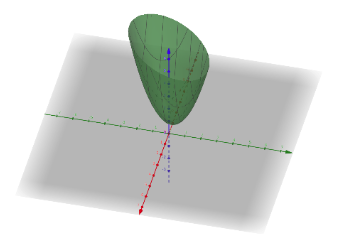
\includegraphics{surface.png}
\end{figure}
\noindent and we are seeking the extreme points enclose within a triangluar area which exists on $D$. We will also search 
for extreme points on the boundaries of this triangular shape. \\\\
\noindent First, we must find the points inside the triangle where there are extremas, aka, when the gradient is $\vec{0}$.\\\\
\noindent $2x - y = 0 \rightarrow y = 2x$\\\\
\noindent $2y - x = 0 \rightarrow x = 0\text{, } y = 0$\\\\
\noindent $\mathbf{point of interest: }D(0,0) = 1$\\\\
\noindent Next, we will test the boundary points by applying three constraints to $D$: the three sides of the triangular shape.\\\\
\noindent $D(0, y) = y^{2} + 1$\\
\noindent $\frac{dD}{dy} = 2y$\\
\noindent $2y = 0 \rightarrow \mathbf{point of interest: } D(0, 0) = 1$\\\\
\noindent $D(x, 4) = x^{2}-4x+17$\\
\noindent $\frac{dD}{dx} =2x -4$\\
\noindent $2x -4 = 0 \rightarrow x = 2$\\
\noindent $\mathbf{point of interest: } D(2, 4) = 13$\\\\
\noindent $D(x, x) = x^{4}+1$\\
\noindent $\frac{dD}{dx} =4x^{3}$\\
\noindent $4x^{3} = 0 \rightarrow x = 0$\\
\noindent $\mathbf{point of interest: } D(0, 0) = 1$\\\\
\noindent Finally, we will exhaust our search by testing the three corners of the triangle.\\\\
\noindent $D(0,0) = 1$, \hspace{10pt} $D(0,4) = 17$, \hspace{10pt} $D(4, 4) = 17$\\\\
\noindent We conclude that within the triangular area, $D$ has an absolute minimum at the origin and absolute maxima at points $(0,4)$ and $(4,4)$.\\\\

\noindent 52.) The minimization of the distance between the point $(2, -1, 1)$ and the plane $x+y-z = 2$ can be obtained as follows.\\\\
\noindent Our goal is to maximize the distance function $d = \sqrt{(x_{1} - x_{0})^{2} + (y_{1} - y_{0})^{2} + (z_{1} - z_{0})^{2}}$\\
\noindent Since $\sqrt{n}$ and $n$, $n \in \mathbb{R}$ are monotonically increasing functions, we can proceed with using $f = d^{2}$.\\\\
\noindent We have the constrants $g = x+y-z$.\\\\
\noindent I'll evaluate $f$ in the following way: find the distance from the point by evaulating $f$ at the point, but apply the constrains 
that $g$ yeilds. $g$ is a function of two variables which we will solve for $z$. We can interpret $g$ as a $z$ depending on $x$ and $y$, so 
that is the $z$ coordinate I'll restrict $f$ to.\\\\
\noindent $f(x,y) = (x-2)^{2} + (y+1)^{2} + (x + y +1)^{2} = 2x^{2}+2y^{2}+2xy-2x+4y+6$\\\\
\noindent Now I'll need to locate the extrema of $f$, specifically, the local minima. We know that it has at least one since it's monotonically increasing. \\\\
\noindent $\frac{\partial f}{\partial x} = 4x+2y-2$\\\\
\noindent $\frac{\partial f}{\partial y} = 4y+2x + 4$\\\\
\noindent $4x+2y+4 = 0 \rightarrow x = -\frac{1}{2}y+\frac{1}{2}$\\\\
\noindent $4y+2x + 4$\\
\noindent $4y -y + 1 +4 = 0 \rightarrow y = -\frac{5}{3}$\\\\
\noindent $4y+2x+4 = 0$\\
\noindent $4[-\frac{5}{3}] + 2x = -4$\\\\
\noindent $x = 2[-\frac{12}{3} + \frac{20}{3}] = \frac{4}{3}$\\\\
\noindent I'll compute the Hessian determinant to test if the point $(\frac{4}{3}, -\frac{5}{3})$ is a minimum.\\
\noindent $\mathbf{H} = f_{xx}f_{yy} - f_{yx}^{2} = (4)(4) - 2 > 0$\\\\
\noindent Since $\mathbf{H} > 0$ and the seconds partials at the critical point are both positive, we can conclude that $(\frac{4}{3}, -\frac{5}{3})$
is the local minimum of the function $f$ with the applied restrictions of $g$. So, this point, which is on the plane $g$, yeilds the smallest value for $f$.
Let's see what that value, the minimized distance, is.\\\\
\noindent  $d = \sqrt{2x^{2}+2y^{2}+2xy-2x+4y+6} 
\\ d =\sqrt{2(\frac{4}{3})^{2}+2(-\frac{5}{3})^{2}+2(\frac{4}{3})(-\frac{5}{3})-2(\frac{4}{3})+4(-\frac{5}{3})+6} = \frac{2\sqrt{3}}{3}$\\\\


\subsection*{Section 14.8}
\noindent 2.) I'll obtain the extreme values of $f = xy$ on the circle $g = x^{2} + y^{2} -10 = 0$ by using the method of Lagrange multipliers.\\\\
\noindent The extreme values exist where the two graphs are touching. We know that if the two graphs are touching, then their gradients are proportional. 
I'll set up the Lagrange muliplier $\lambda$ as the proportionality constant: \\\\
\noindent $\nabla f \propto \nabla g \rightarrow \nabla f = \lambda \nabla g$\\
\noindent $ \langle y, x\rangle = \lambda \langle 2x, 2y\rangle$\\\\
\noindent Now we can equate coefficients and use the constrain equation.\\
\noindent $y = 2\lambda x$, \hspace{10pt} $x = 2y\lambda$\\
\noindent $x = 2\lambda (2x\lambda) \rightarrow \lambda = \pm \frac{1}{2}$\\
\noindent Let's test the $\lambda = \frac{1}{2}$ case.\\
\noindent $y = 2x(\frac{1}{2}) = x$\\
\noindent $x^{2} + y^{2} = 10$\\
\noindent $x^{2} + \frac{1}{4} = 10 \rightarrow x = \pm\sqrt{5}$\\
\noindent When $x = -\sqrt{5}$, $y = -\sqrt{5}$. When $x = -\sqrt{5}$, $y = -\sqrt{5}$.\\
\noindent Let's test the $\lambda = -\frac{1}{2}$ case.\\
\noindent $y = 2x(-\frac{1}{2}) = -x$\\
\noindent $x^{2} = y^{2} = 10 \rightarrow x = \pm\sqrt{5}$\\
\noindent When $x = -\sqrt{5}$, $y = \sqrt{5}$. When $x = \sqrt{5}$, $y = -\sqrt{5}$.\\
\noindent The points at which the gradients are proportional, where the functions are tangentially touching,
 are $(\pm \sqrt{5}, \sqrt{5})$ and $(\pm \sqrt{5}, -\sqrt{5})$.\\\\

\noindent 4.) I'll obtain the extreme values of $f = x^{2}y$ on $g = x+y=3$ by using the method of Lagrange mulitpliers.\\\\
\noindent Again, the funtions are touching tangentially at the extreme points. Set up the Lagrange multiplier using the Orthogonal Gradient Theorem. 
\noindent $\nabla f \propto \nabla g \rightarrow \nabla f = \lambda \nabla g$\\
\noindent $ \langle 2xy,x^{2}\rangle = \lambda \langle 1, 1\rangle$\\\\
\noindent Equate coefficients now. $2xy = \lambda$, \hspace{10pt} $x^{2} = \lambda$\\
\noindent $2xy = x^{2} \rightarrow x(2y -x) = 0$\\
\noindent What happens if $x = 0$:
\noindent Using the $g$ equation, $x + y = 3 \rightarrow y = 3$\\
\noindent What happens if $2y -x$ is zero:
\noindent $2y = x \rightarrow y = \frac{1}{2}x$\\
\noindent $(\frac{1}{2}x) + x = 3 \rightarrow x = 3$, $y = 1$\\
\noindent So, the functions are touching at the points $(3, 1) = 0$ and $(2, 1) = 4$ and these two points are the extremas. \\\\
\noindent 8.) I'll find the points on $f = x^{2}+xy+y^{2} = 1$ contained in an $x-y$ plane nearest and farthest from the origin. I'll use Lagrange muliplers again.\\\\
\noindent The extreme points are located on the curve and the plane simultaneosly. I'll use the Orthogonal Gradient Theorem.\\
\noindent $\nabla f \propto \nabla g \rightarrow \nabla f = \lambda \nabla g$\\
\noindent $ \langle 2x,2y\rangle = \lambda \langle 2x+y, x+2y\rangle$\\\\
\noindent Equate coefficients. $2x = 2\lambda x +\lambda y$, \hspace{10pt} $2y = 2\lambda y + \lambda x$\\
\noindent $\lambda = \frac{2x}{2x+y}$, \hspace{10pt} $\lambda = \frac{2y}{2y+x}$\\
\noindent $(2x+y)(2y+x)[\frac{2x}{2x+y} = \frac{2y}{2y+x}]$\\
\noindent $x(2y+x) = y(2x+y)$\\
\noindent $x^{2} + 2xy  = y^{2}+ 2xy \rightarrow x = \pm x$\\
\noindent When $y = x$, then $x^{2} + x(x) + (x)^{2} = 1$.\\
\noindent $3x^{2} = 1 \rightarrow x = \pm \frac{\sqrt{3}}{3}$ yeilds points $(\pm \frac{\sqrt{3}}{3}, \pm \frac{\sqrt{3}}{3})$.\\
\noindent When $y =-x$, then $x^{2} + x(-x) + (-x)^{2} = 1$.\\
\noindent $x^{2} = 1 \rightarrow x = \pm 1$ yeilds points $(\pm 1, \mp 1)$.\\
\noindent Now I'll need to determine if these points are minima or maxima.\\
\noindent $f(-1, 1) = 2$, \hspace{10pt} $f(1, -1) = 2$, \hspace{10pt} $f(\frac{\sqrt{3}}{3}, \frac{\sqrt{3}}{3}) = \frac{2}{3}$, \hspace{10pt} $-f(\frac{\sqrt{3}}{3}, -\frac{\sqrt{3}}{3}) = \frac{2}{3}$\\
\noindent In conclusion, the points  $(\pm 1, \mp 1)$ are farthest away from the origin and the points $(\pm \frac{\sqrt{3}}{3}, \pm \frac{\sqrt{3}}{3})$ are the closest.\\\\

\noindent 24.) Using Lagrange Mulipliers, I'll find the extreme points that a sphere $g = x^{2} + y^{2} + z^{2} = 25$ has in common with $f = x+2y + 3z$'s extreme points.\\\\
\noindent Set up the Orhogonal Gradient theorem equation and equate coefficients. \\
\noindent $\nabla f \propto \nabla g \rightarrow \nabla f = \lambda \nabla g$\\
\noindent $ \langle 1, 2, 3\rangle = \lambda \langle 2x, 2y, 2z\rangle$\\\\
\noindent $x = \frac{1}{2\lambda}$, \hspace{10pt} $y = \frac{1}{\lambda}$, \hspace{10pt} $z = \frac{1}{2}\lambda$\\
\noindent By inspection, it appears that $y = 2x$ and $z = 3x$. So, I'll plug these into the sphere equqation to obtain the value of x.\\
\noindent $x^{2} + (2x)^{2} + (3x)^{2} = 25$\\
\noindent $x = \pm \frac{5\sqrt{14}}{14}$ yeilds two points of interest. Namely: \\
\noindent $(\pm \frac{5\sqrt{14}}{14}, \pm \frac{10\sqrt{14}}{14}, \pm \frac{15\sqrt{14}}{14})$
\noindent $f(- \frac{5\sqrt{14}}{14}, - \frac{10\sqrt{14}}{14},  -\frac{15\sqrt{14}}{14}) = -5\sqrt{14}$\\
\noindent $f( \frac{5\sqrt{14}}{14},  \frac{10\sqrt{14}}{14},  \frac{15\sqrt{14}}{14}) = 5\sqrt{14}$\\
\noindent $(\frac{5\sqrt{14}}{14},  \frac{10\sqrt{14}}{14},  \frac{15\sqrt{14}}{14})$ is the common maximum and $(- \frac{5\sqrt{14}}{14}, - \frac{10\sqrt{14}}{14},  -\frac{15\sqrt{14}}{14})$ is the common minimum. \\\\

\noindent 26.) The goal is to minimize the product $f = xyz$ as long as $g = x + y + z^{2} = 16$. Let's use Lagrange Mulipliers.\\\\
\noindent Set up the proportion, since the two functions' gradients are proportional at their minima (since they are touching in one or more locations).
\noindent $\nabla f \propto \nabla g \rightarrow \nabla f = \lambda \nabla g$\\
\noindent $ \langle yz, xz, xy\rangle = \lambda \langle 1, 1, 2z\rangle$\\\\
\noindent $yz = \lambda$ (I), \hspace{10pt} $xz = \lambda$ (II), \hspace{10pt} $xy = 2\lambda z$(III)\\
\noindent $yz = xz$\\
\noindent $yz - xz = 0$\\
\noindent $z(y -x) = 0$\\
\noindent What happens if $z$ is zero: \\
\noindent $\rightarrow \leftarrow$ $z$ has to be $> 0$ because I'm assuming $(I)$ and $(II)$ are true statements.\\
\noindent $y = x$ (*)\\
\noindent $x^{2} = 2\lambda z$, \hspace{10pt} $xz = \lambda$\\
\noindent $x^{2} = 2(xz)z$\\
\noindent $x(x - 2z^{2}) = 0$\\
\noindent Since I'm assuming (III), $x \neq 0$, so $x = 2z^{2} = y$ from (*).\\
\noindent Using the constraint: $2z^{2} + 2z^{2} = z^{2} = 16 \rightarrow z = \pm \frac{4\sqrt{5}}{5}$, but I know that $z = \frac{4\sqrt{5}}{5}$ only. \\
\noindent When $z = \frac{4\sqrt{5}}{5}$, $y = x = \frac{35}{5}$\\
\noindent $f(\frac{32}{5}, \frac{32}{5}, \frac{4\sqrt{5}}{5}) = \frac{4096\sqrt{5}}{125}$ is the minimum product that sastisfies the constraint. Neat! \bcsmbh


\end{document}
